\documentclass[11pt]{article}

\usepackage{graphicx}
\usepackage{wrapfig}
\usepackage{url}
\usepackage{wrapfig}
\usepackage{color}
\usepackage{marvosym}
\usepackage{enumerate}
\usepackage{subfigure}
\usepackage{tikz}
\usepackage{amsmath}
\usepackage{amssymb}
\usepackage{hyperref} 


\oddsidemargin 0mm
\evensidemargin 5mm
\topmargin -20mm
\textheight 240mm
\textwidth 160mm




\newcommand{\vw}{{\bf w}}
\newcommand{\vx}{{\bf x}}
\newcommand{\vy}{{\bf y}}
\newcommand{\vxi}{{\bf x}_i}
\newcommand{\yi}{y_i}
\newcommand{\vxj}{{\bf x}_j}
\newcommand{\vxn}{{\bf x}_n}
\newcommand{\yj}{y_j}
\newcommand{\ai}{\alpha_i}
\newcommand{\aj}{\alpha_j}
\newcommand{\X}{{\bf X}}
\newcommand{\Y}{{\bf Y}}
\newcommand{\vz}{{\bf z}}
\newcommand{\msigma}{{\bf \Sigma}}
\newcommand{\vmu}{{\bf \mu}}
\newcommand{\vmuk}{{\bf \mu}_k}
\newcommand{\msigmak}{{\bf \Sigma}_k}
\newcommand{\vmuj}{{\bf \mu}_j}
\newcommand{\msigmaj}{{\bf \Sigma}_j}
\newcommand{\pij}{\pi_j}
\newcommand{\pik}{\pi_k}
\newcommand{\D}{\mathcal{D}}
\newcommand{\el}{\mathcal{L}}
\newcommand{\N}{\mathcal{N}}
\newcommand{\vxij}{{\bf x}_{ij}}
\newcommand{\vt}{{\bf t}}
\newcommand{\yh}{\hat{y}}
\newcommand{\code}[1]{{\footnotesize \tt #1}}
\newcommand{\alphai}{\alpha_i}

\pagestyle{myheadings} 
\markboth{Homework 7}{Fall 2012 CS 475 Machine Learning: Homework 7} 


\title{CS 475 Machine Learning: Homework 7\\Graphical Models \\
\Large{Due: Wednesday November 28, 2012, 12pm}\\
100 Points Total \hspace{1cm} Version 1.0}

\author{}
\date{}

\begin{document}
\large
\maketitle
\thispagestyle{headings}

\vspace{-.5in}

\section{Programming (55 points)}
In this assignment you will implement a Markov Random Field for image denoising. Refer to section 8.3.3 of the book for details on how to define and update the parameters of the model. See figure 8.31 for the structure of the network. This writeup provides additional details needed for your implementation.

\subsection{Image Processing Tools}
As part of this assignment you will use a provided Java library for image processing. The distributed code contains three classes with main methods:
\begin{itemize}
\item \code{cs475.image\_denoise.InsertImageNoise}: Insert random noise into an image by randomly permuting pixels in an image. We provide images that have been permuted, but you can use this class to create new images for testing.
\item \code{cs475.image\_denoise.RemoveImageNoise}: Remove image noise (denoise an image) using a Markov Random Field. This class calls \code{cs475.image\_denoise.MRFImageProcessor}, which is where you will implement your MRF.
\item \code{cs475.image\_denoise.CompareImages}: This class compares two images by comparing the pixel values of each image.

For images with 2 colors, the two images will be compared by measuring the exact match between pixel values. If every pixel in each image contains the identical color value, the accuracy will be 100\%. If no pixels in the two images have the same value, the accuracy will be 0\%. 

For greyscale images, the comparison measures the average distance between the pixels in the two images. The distance between two pixels is a function of the distance between the colors of each pixel. Note that while smaller distances mean that the two images are more similar, you should not interpret the relative differences between two images compared to a baseline as success in denoising the image. In fact, an image may have a greater distance to the original image but be less noisy. You can verify your results by examining the image to see if the noise has been removed. To evaluate your code, we will compare your results to a correct implementation.
\end{itemize}

You can run each of these main methods without arguments to see a description of the command line options.

In addition to these three classes, \code{cs475.image\_denoise.ImageUtils} contains common image processing methods that are used by multiple classes. You may find it helpful to use methods defined in this class.

You should not modify any of the above classes, nor should you need to create new files. All of your code should be written in \code{cs475.image\_denoise.MRFImageProcessor}. The method \code{MRFImageProcessor.denoisifyImage} will decide which MRF algorithm to run depending on the input (see below). Using the descriptions below, you should check the input to see which MRF to use (i.e., check the number of colors in the image and the number of images provided.) You may check the number of colors in an image using the method \code{ImageUtils.countColors(int[][] image)}, which returns the number of colors in a provided image. You can also get the max color index in an image using the method \code{ImageUtils.maxColor(int[][] image)}.


\subsection{Data}
We are providing several images you may use for image processing. For each image, we provide a clean and at least one noisy version of the image. You are welcome to create more noisy versions or to use other images (make sure they are greyscale \code{bmp} images). 

You should run \code{RemoveImageNoise} on the noisy image and compare the result to the image without noise. While you can use the provided 
class \code{CompareImages}, you may also find it helpful to visually inspect the images in a standard image viewer.

There are two synthetic images: easy and hard.
\begin{itemize}
\item {\bf Easy}: It should be simple to remove most noise from these images and you should expect your MRF to denoisify these images almost completely correctly.
\item {\bf Hard}: These images contain random pixel values so it will be impossible for your MRF to denoisify this image. You should expect random accuracy when compared with the clean image.
\end{itemize}

While the code supports many image formats you should only use \code{bmp} files (extensions that end in \code{.bmp}). The use of other formats will cause problems with your code since various types of compression are used in other formats.

\subsection{Running the Algorithm}
You will implement iterated conditional modes, an iterative algorithm that updates each hidden node in the model individually. Since your output must match our implementation, you need to update the hidden nodes in a specified order. Each of your implementations should iterate over the hidden nodes as follows:
\begin{verbatim}
for (int ii = 0; ii < hidden_nodes.length; ii++) {
    for (int jj = 0; jj < hidden_nodes[ii].length; jj++) {
        // Update hidden_nodes[ii][jj]
    }
}
\end{verbatim}
where \code{hidden\_nodes[ii][jj]} ($\vx$) corresponds to the observed variable \code{image[ii][jj]} ($\vy$). The update selects the color for hidden node $ii,jj$ that maximizes the energy function. Additionally, you should initialize your hidden variables $\vx$ to be the same as the observed variables $\vy$.
%When given two images (see section \ref{sec:single_two_images}), use the first image to initialize your variables.

As in the book, we will assume the bias term has the value $h=0$ for all models in this assignment. 

The run time for this code should be pretty fast. I expect about 30 seconds per iteration for the greyscale images.

\subsection{Output}
The output of your code should be the values of the nodes $\vx$, which represents the denoisified image. The values for these nodes are stored in a \code{int[][]} object and should be returned at the end of the \code{MRFImageProcessor.denoisifyImage} method you will implement. You are not required to print any output in this assignment. The provided code will read and output the images. 

\subsection{MRFs for Black and White Images}
Section 8.3.3 of the book describes a MRF for black and white images (2 pixels). When provided a single image with 2 pixels, you will use this algorithm with two small changes:
\begin{itemize}
\item The energy function for the clique between hidden nodes $x_i$ and $x_j$ is given by:
\[
\psi_N(x_i, x_j) = -\beta~~\textrm{if}~~ x_i = x_j, \beta~~ \textrm{otherwise.}
\]
\item The energy function for the clique between a hidden node $x_i$ and an observed node $y_i$ is given by:
\[
\psi_O(x_i, y_i) = -\eta ~~ \textrm{if}~~ x_i = y_i, \eta~~ \textrm{otherwise.}
\]
\end{itemize}
Note that this is the same as the book except you should not expect the colors to have values $+1$ and $-1$. Instead, you will have different integer values as colors.

For this model, on \code{easy.1.2\_colors.bmp} with $\eta=2.1$, $\beta=2.0$ and $num\_iterations=20$ you should obtain 100\% accuracy. With the same parameters on \code{easy.2.2\_colors.bmp} you should obtain accuracy above 99.99\% accuracy. The running time of both of these tests should be a few seconds.

For other images, you may experiment with different values of $\eta$ and $\beta$. The values of $\eta=2.1$ and $\beta=1.0$ described in the book are a good starting point for exploration.

You should implement this model in \code{MRFImageProcessor} and it should be run when you are given a single image with only 2 colors. You may check the number of colors in an image using the method \code{ImageUtils.countColors(int[][] image)}, which returns the number of colors in a provided image.

This model should be used for any single image with only 2 colors.

\subsection{MRFs for Greyscale Images}
Extend your implementation of a single layer MRF to greyscale images. If you receive an image with more than 2 colors, assume it is a greyscale image. For greyscale images, the energy functions should be
\[
\psi_N(x_i, x_j) = [\log (|x_j -x_i| +1) -1] \beta ~,
\]
and
\[
\psi_O(x_i, y_i) = [\log (|x_i - y_i| +1) -1] \eta ~.
\]

%%%%%%%%%%%%%%%%%%%%%%%%%%%%%%%%%%%%%%%%%%%%%%%%%%%%%%%%%%%%%%%%%%%%%%%%%%%%%%%%%%%%
\subsection{MRFs with Non-Local Information}
This MRF is identical to the previous ones except it has an extra layer of nodes above the $\vx$ nodes, which we will call $\vz$ nodes. These nodes will allow for more non-local smoothing because they introduce more non-local edges.

Each node $z \in \vz$ will be connected a set of nodes $\vx$ but not to any other node $z' \in \vz$ or $y \in \vy$. Begin by dividing $\vx$ into $K \times K$ blocks, where $K$ is a parameter you will supply (default 4). For example, node $x_{i,j}$ will be in the first block if $0 \le i < K$ and $0 \le j < K$. Depending on the size of the image, you may have blocks at the end of the image that are smaller than $K \times K$. All nodes $\vx$ in the same block will be connected to the same $z$. This means that each $z$ will have connections to $K^2$ $\vx$-nodes but to no other node.

Generally speaking, assume in any one dimension (i.e. \emph{horizontal} or \emph{vertical}) you have $x_1, x_2, ..., x_n$ and $z_1, z_2, ..., z_m$, and $m \leq n$. Use the following rule to determine the connection between $\vz$ and $\vx$ nodes:
\[
x_i \textrm{ is connected to } z_j \textrm{ , where } \lfloor \frac{i}{K} \rfloor = j
\]
This applies in both dimensions, \emph{horizontal} and \emph{vertical}. This formula must be applied jointly in each dimension. 

In addition to the previous energy functions $\psi_O$ and $\psi_N$, we will now also have:
\[
	\psi_H(x_i, z_j) = - \omega \text{ if } x_i = z_j \text{, } \omega \text{ otherwise}
\]
in the black and white case, and
\[
	\psi_H(x_i, z_j) = [\log (|x_i - z_j| +1) -1] \omega
\]
in the greyscale case.

$\omega$ is a parameter which you can try different values for. It might be good to start with values less than $\eta$ and $\beta$, since many more nodes are connected to each $z$, and increase it gradually. Your output will be the same as above, i.e. you need only output the $\vx$ nodes.

As before, the order you update the nodes matters. For this model, the initial values for the nodes $\vz$ should be the average of all the nodes connected to them. Note that this average will be a majority vote in the case of black and white images, where the lower indexed value is selected in case of a tie. When you update the nodes, first update all nodes $\vx$ and then update all nodes $\vz$ as:


\begin{verbatim}
// Update hidden_nodes as above

for (int ii = 0; ii < z_nodes.length; ii++) {
    for (int jj = 0; jj < z_nodes[ii].length; jj++) {
        // Update z_nodes[ii][jj]
    }
}
\end{verbatim}

This two hidden level MRF will be used when the $\code{use\_second\_level}$ command line option is provided. $\omega$ is provided on the command line just like $\eta$ and $\beta$. The window size $K$ is set with the command line option $\code{num\_K}$.

\subsection{Additional Facts}
\begin{itemize}
\item We will only give you valid images. Images will have arrays of uniform length (so you can iterate over them without a problem.) All colors will be non-negative integers.
\item In case of a tie between two colors for maximizing the energy function, select the lowest indexed color.
\item {\bf IMPORTANT}: We will use a strategy where we fix all hidden nodes until after the full iteration is complete. This means that when you update the value of hidden node $ii,jj$, don't use this new value until the iteration is complete. This means you should save the new values and old values until you are ready to update after a full iteration.
\end{itemize}


\section{Analytical (45 points)}
\paragraph{1. (10 points)} Consider the Bayesian Network given in Figure \ref{dgm}. Are the sets ${\bf A}$ and ${\bf B}$ d-separated given set ${\bf C}$ for each of the following definitions of ${\bf A}$, ${\bf B}$ and ${\bf C}$? Justify each answer.
\begin{enumerate}[a.]
\item ${\bf A} = \{x_1\}$, ${\bf B} = \{x_9\}$, ${\bf C} = \{x_5,x_{14}\}$
\item ${\bf A} = \{x_{11}\}$, ${\bf B} = \{x_{13}\}$, ${\bf C} = \{x_1,x_{15}\}$
\item ${\bf A} = \{x_4\}$, ${\bf B} = \{x_5\}$, ${\bf C} = \{x_{10},x_{16}\}$
\item ${\bf A} = \{x_3, x_4\}$, ${\bf B} = \{x_{13},x_9\}$, ${\bf C} = \{x_{10},x_{15},x_{16}\}$
\end{enumerate}
Now consider a Markov Random Field in Figure \ref{ugm}, which has the same structure as the previous Bayesian network.  Re-answer each of the above questions with justifications for your answers.

\newcommand{\nodesize}{.6}
\begin{figure}[h]
\centering
\subfigure[Directed Graphical Model]{
\begin{tikzpicture}[style=thick,scale=1] 
\begin{scope}[shape=circle,minimum size=0.1cm] 
\tikzstyle{every node}=[draw,fill] 
\node[fill=none,scale=\nodesize] (X_1) at (2,4) {$\mathbf{X_1}$};
\node[fill=none,scale=\nodesize] (X_2) at (4,4) {$\mathbf{X_2}$};
\node[fill=none,scale=\nodesize] (X_3) at (0,3) {$\mathbf{X_3}$};
\node[fill=none,scale=\nodesize] (X_4) at (2,3) {$\mathbf{X_4}$};
\node[fill=none,scale=\nodesize] (X_5) at (4,3) {$\mathbf{X_5}$};
\node[fill=none,scale=\nodesize] (X_6) at (1,2) {$\mathbf{X_6}$};
\node[fill=none,scale=\nodesize] (X_7) at (3,2) {$\mathbf{X_7}$};
\node[fill=none,scale=\nodesize] (X_8) at (4,2) {$\mathbf{X_8}$};
\node[fill=none,scale=\nodesize] (X_9) at (5,2) {$\mathbf{X_9}$};
\node[fill=none,scale=\nodesize] (X_10) at (0,1) {$\mathbf{X_{10}}$};
\node[fill=none,scale=\nodesize] (X_11) at (1,1) {$\mathbf{X_{11}}$};
\node[fill=none,scale=\nodesize] (X_12) at (2,1) {$\mathbf{X_{12}}$};
\node[fill=none,scale=\nodesize] (X_13) at (4,1) {$\mathbf{X_{13}}$};
\node[fill=none,scale=\nodesize] (X_14) at (5,1) {$\mathbf{X_{14}}$};
\node[fill=none,scale=\nodesize] (X_15) at (1,0) {$\mathbf{X_{15}}$};
\node[fill=none,scale=\nodesize] (X_16) at (3,0) {$\mathbf{X_{16}}$};
\draw [->] (X_1) -- (X_3);
\draw [->] (X_2) -- (X_5);
\draw [->] (X_4) -- (X_3);
\draw [->] (X_3) -- (X_6);
\draw [->] (X_4) -- (X_6);
\draw [->] (X_5) -- (X_9);
\draw [->] (X_5) -- (X_8);
\draw [->] (X_6) -- (X_10);
\draw [->] (X_6) -- (X_11);
\draw [->] (X_7) -- (X_12);
\draw [->] (X_8) -- (X_12);
\draw [->] (X_8) -- (X_13);
\draw [->] (X_9) -- (X_14);
\draw [->] (X_11) -- (X_15);
\draw [->] (X_12) -- (X_15);
\draw [->] (X_12) -- (X_16);
\draw [->] (X_14) -- (X_16);
\end{scope} 
\end{tikzpicture}
\label{dgm}
}
\subfigure[Undirected Graphical Model]{
\begin{tikzpicture}[style=thick,scale=1] 
\begin{scope}[shape=circle,minimum size=0.1cm] 
\tikzstyle{every node}=[draw,fill] 
\node[fill=none,scale=\nodesize] (X_1) at (2,4) {$\mathbf{X_1}$};
\node[fill=none,scale=\nodesize] (X_2) at (4,4) {$\mathbf{X_2}$};
\node[fill=none,scale=\nodesize] (X_3) at (0,3) {$\mathbf{X_3}$};
\node[fill=none,scale=\nodesize] (X_4) at (2,3) {$\mathbf{X_4}$};
\node[fill=none,scale=\nodesize] (X_5) at (4,3) {$\mathbf{X_5}$};
\node[fill=none,scale=\nodesize] (X_6) at (1,2) {$\mathbf{X_6}$};
\node[fill=none,scale=\nodesize] (X_7) at (3,2) {$\mathbf{X_7}$};
\node[fill=none,scale=\nodesize] (X_8) at (4,2) {$\mathbf{X_8}$};
\node[fill=none,scale=\nodesize] (X_9) at (5,2) {$\mathbf{X_9}$};
\node[fill=none,scale=\nodesize] (X_10) at (0,1) {$\mathbf{X_{10}}$};
\node[fill=none,scale=\nodesize] (X_11) at (1,1) {$\mathbf{X_{11}}$};
\node[fill=none,scale=\nodesize] (X_12) at (2,1) {$\mathbf{X_{12}}$};
\node[fill=none,scale=\nodesize] (X_13) at (4,1) {$\mathbf{X_{13}}$};
\node[fill=none,scale=\nodesize] (X_14) at (5,1) {$\mathbf{X_{14}}$};
\node[fill=none,scale=\nodesize] (X_15) at (1,0) {$\mathbf{X_{15}}$};
\node[fill=none,scale=\nodesize] (X_16) at (3,0) {$\mathbf{X_{16}}$};
\draw [-] (X_1) -- (X_3);
\draw [-] (X_2) -- (X_5);
\draw [-] (X_3) -- (X_4);
\draw [-] (X_3) -- (X_6);
\draw [-] (X_4) -- (X_6);
\draw [-] (X_5) -- (X_9);
\draw [-] (X_5) -- (X_8);
\draw [-] (X_6) -- (X_10);
\draw [-] (X_6) -- (X_11);
\draw [-] (X_7) -- (X_12);
\draw [-] (X_8) -- (X_12);
\draw [-] (X_8) -- (X_13);
\draw [-] (X_9) -- (X_14);
\draw [-] (X_11) -- (X_15);
\draw [-] (X_12) -- (X_15);
\draw [-] (X_12) -- (X_16);
\draw [-] (X_14) -- (X_16);
\end{scope} 
\end{tikzpicture}
\label{ugm}
}
\caption{Two graphs are the same. However since (a) is directed and (b) is undirected the two graphs have different a conditional independence interpretation.}
\end{figure}

\paragraph{2. (5 points)} Let $X = (X_1, . . . , X_{10})^T$ be a random vector with distribution given by the graphical model in Figure \ref{dgm}. Consider variable $X_2$. What is the minimal subset of the variables, $A\subset \mathcal{X} -\{X_2\}$, such that $X_2$ is independent of the rest of the variables ($\mathcal{X} - (A\cup{\{ X_2\}}$)) given A? Justify your answer.

\paragraph{3. (10 points)} Let $X = (X_1, . . . , X_{d}^T)$ be a random vector with a $d$-variate Gaussian distribution $N(0,\Sigma)$. Define the precision matrix as $\Omega = \Sigma^{-1}$. Please prove that $\Omega_{ij}=0$ implies the conditional independence between $X_i$ and $X_j$ given the remaining variables, i.e., a sparsity pattern $\Omega$ is equivalent to an adjacency matrix of a Gaussian Markov random filed.

Such a phenomenon enables us to estimate the unknown structure of a Gaussian Markov random filed by maximizing the penalized Gaussian likelihood,
\begin{align}\label{glasso}
\hat{\Omega} = \arg\max_{\Omega} \log \rm{det}(\Omega) - {\rm tr}(S\Omega) - \lambda\sum_{j<k}|\Omega_{jk}|,
\end{align}
where ${\rm det}(\cdot)$ denotes the determinant of the matrix, and ${\rm tr}(\cdot)$ denotes the trace of the matrix. \eqref{glasso} is well known as the graphical lasso, which means ``the lasso for Gaussian graphical models".

\paragraph{4. (10 points)} The Naive Bayes model assumes that all features in a $m$-dimensional vector $X$ are conditionally independent on each other given the label $Y$. A Naive Bayes classifier can be represented as a graphical model (figure \ref{fig:nb}). Notice that the nodes for $X$ are shaded since they are observed. The variable $Y$ is observed during training but is unobserved at test time.

\begin{figure}[h]
	\begin{center}
		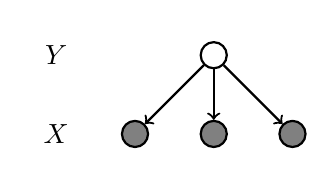
\begin{tikzpicture}[style=thick] 
			\begin{scope}[shape=circle,minimum size=0.25cm] 
			\tikzstyle{every node}=[draw,fill] 
			\node[fill=none,draw=none] at (-1,0) {$X$};
			\node[fill=none,draw=none] at (-1,1) {$Y$};
			
			\node[fill=none] (root) at (1,1) {};
			\foreach \x in {0,1,2} {
				\node[fill=gray] (q_\x) at (\x,0) {};
			}
			\end{scope} 
			\foreach \x in {0,1,2} {
				\draw [->] (root) -- (q_\x);
			}	 
		\end{tikzpicture}
	\end{center}
	\caption{The graphical model for the Naive Bayes classifier.}
	\label{fig:nb}
\end{figure}

The Naive Bayes model data likelihood is defined by:
\begin{align}
P(Y_i,X_i) = \prod_{i=1}^n P(Y_i,X_i) = \prod_{i=1}^n \prod_{j=1}^m P(X_{ij}|Y_i)P(Y_i),
\end{align}

Now we consider a semi-supervised learning scheme with $n$ observations, in which $X$ is observed for all training examples, while $Y$ is partially observed, i.e., some training examples have their $Y$'s missing. We will call the set containing the first type of examples $L$ (labeled) and the set containing the second type of examples $U$ (unlabeled.)  Since some of labels $Y_i$ are missing (those in $U$ but not those in $L$), we cannot maximize the joint distribution $P(Y,X)$ directly. Instead, we must maximize the likelihood function using just the examples $X$: $P(X)$.

Please derive an EM algorithm for maximizing the likelihood function $P(X)$ on both the labeled and unlabeled data ($L+U$). Your solution should include the likelihood function $P(X)$ and both the E-step and the M-step of the algorithm.

\paragraph{5. (10 points)} Consider the factor graph in Figure \ref{fig:factor_graph}. Can the Max Product algorithm be used to compute the maximal assignment in this network?
\newcommand{\factorsize}{1}
\begin{figure}[h]
	\begin{center}
\begin{tikzpicture}[style=thick,scale=1] 
			\begin{scope}[shape=circle,minimum size=0.1cm] 
			\tikzstyle{every node}=[draw,fill] 
			\node[fill=none,scale=\nodesize] (X_1) at (2,4) {$\mathbf{X_1}$};
			\node[fill=none,scale=\nodesize] (X_2) at (4,4) {$\mathbf{X_2}$};
			\node[fill=red,scale= \factorsize,shape=rectangle] (X_3) at (0,3) {};
			\node[fill=none,scale=\nodesize] (X_4) at (2,3) {$\mathbf{X_4}$};
			\node[fill=red,scale=\factorsize,shape=rectangle] (X_5) at (4,3) {};
			\node[fill=none,scale=\nodesize] (X_6) at (1,2) {$\mathbf{X_6}$};
			\node[fill=none,scale=\nodesize] (X_7) at (3,2) {$\mathbf{X_7}$};
			\node[fill=none,scale=\nodesize] (X_8) at (4,2) {$\mathbf{X_8}$};
			\node[fill=none,scale=\nodesize] (X_9) at (5,2) {$\mathbf{X_9}$};
			\node[fill=red,scale= \factorsize,shape=rectangle] (X_10) at (0,1) {};
			\node[fill=red,scale= \factorsize,shape=rectangle] (X_11) at (1,1) {};
			\node[fill=red,scale= \factorsize,shape=rectangle] (X_12) at (2,1) {};
			\node[fill=red,scale= \factorsize,shape=rectangle] (X_13) at (4,1) {};
			\node[fill=red,scale= \factorsize,shape=rectangle] (X_14) at (5,1) {};
			\node[fill=none,scale=\nodesize] (X_15) at (1,0) {$\mathbf{X_{15}}$};
			\node[fill=none,scale=\nodesize] (X_16) at (3,0) {$\mathbf{X_{16}}$};
			\draw [-] (X_1) -- (X_3);
			\draw [-] (X_2) -- (X_5);
			\draw [-] (X_3) -- (X_4);
			\draw [-] (X_3) -- (X_6);
			\draw [-] (X_4) -- (X_5);
			\draw [-] (X_5) -- (X_7);
			\draw [-] (X_5) -- (X_8);
			\draw [-] (X_6) -- (X_10);
			\draw [-] (X_6) -- (X_11);
			\draw [-] (X_6) -- (X_12);
			\draw [-] (X_7) -- (X_12);
			\draw [-] (X_8) -- (X_12);
			\draw [-] (X_8) -- (X_13);
			\draw [-] (X_9) -- (X_14);
			\draw [-] (X_11) -- (X_15);
			\draw [-] (X_12) -- (X_15);
			\draw [-] (X_12) -- (X_16);
			\draw [-] (X_14) -- (X_16);
			\end{scope} 
		\end{tikzpicture}
		\caption{A Factor Graph}
			\label{fig:factor_graph}
		\end{center}
\end{figure}


\begin{itemize}
\item If the Max Product algorithm {\bf can} be applied, show how it can be applied to compute the marginal $P(X_{16})$ (i.e., write equations). What property enables the max product algorithm to be applied?
\item If the Max Product algorithm {\bf cannot} be applied, show why not (i.e., write equations). Describe an algorithm that can be used to compute the maximal assignment for $P(X_{16})$.
\end{itemize}

\section{What to Submit}
In each assignment you will submit two things.
\begin{enumerate}
\item {\bf Code:} Your code as a zip file named {\tt library.zip}. {\bf You must submit source code (.java files)}. We will run your code using the exact command lines described above, so make sure it works ahead of time. Remember to submit all of the source code, including what we have provided to you.
\item {\bf Writeup:} Your writeup as a {\bf PDF file} (compiled from latex) containing answers to the analytical questions asked in the assignment. Make sure to include your name in the writeup PDF and use the provided latex template for your answers.
\end{enumerate}
Make sure you name each of the files exactly as specified (library.zip and writeup.pdf).

To submit your assignment, visit the ``Homework'' section of the website (\href{http://www.cs475.org/}{http://www.cs475.org/}.)

\section{Questions?}
Remember to submit questions about the assignment to the appropriate group on the class discussion board: \href{http://bb.cs475.org/}{http://bb.cs475.org}.

\end{document}



